\documentclass[a4paper,11pt]{article}
\usepackage{polski}
\usepackage[utf8]{inputenc}
\usepackage{latexsym}
\usepackage{graphicx} 
\usepackage{float}
\usepackage[margin=2cm]{geometry}
\usepackage{lscape}
\usepackage{listings}
\usepackage{color}
\usepackage{underscore}

\definecolor{mygreen}{rgb}{0,0.6,0}
\definecolor{mygray}{rgb}{0.5,0.5,0.5}
\definecolor{mymauve}{rgb}{0.58,0,0.82}

\lstset{ %
  backgroundcolor=\color{white},   % choose the background color; you must add \usepackage{color} or \usepackage{xcolor}; should come as last argument
  basicstyle=\footnotesize,        % the size of the fonts that are used for the code
  breakatwhitespace=false,         % sets if automatic breaks should only happen at whitespace
  breaklines=true,                 % sets automatic line breaking
  captionpos=b,                    % sets the caption-position to bottom
  commentstyle=\color{mygreen},    % comment style
  deletekeywords={...},            % if you want to delete keywords from the given language
  escapeinside={\%*}{*)},          % if you want to add LaTeX within your code
  extendedchars=true,              % lets you use non-ASCII characters; for 8-bits encodings only, does not work with UTF-8
  frame=single,	                   % adds a frame around the code
  keepspaces=true,                 % keeps spaces in text, useful for keeping indentation of code (possibly needs columns=flexible)
  keywordstyle=\color{blue},       % keyword style
  language=VHDL,                 % the language of the code
  morekeywords={*,...},            % if you want to add more keywords to the set
  numbers=left,                    % where to put the line-numbers; possible values are (none, left, right)
  numbersep=5pt,                   % how far the line-numbers are from the code
  numberstyle=\tiny\color{mygray}, % the style that is used for the line-numbers
  rulecolor=\color{black},         % if not set, the frame-color may be changed on line-breaks within not-black text (e.g. comments (green here))
  showspaces=false,                % show spaces everywhere adding particular underscores; it overrides 'showstringspaces'
  showstringspaces=false,          % underline spaces within strings only
  showtabs=false,                  % show tabs within strings adding particular underscores
  stepnumber=2,                    % the step between two line-numbers. If it's 1, each line will be numbered
  stringstyle=\color{mymauve},     % string literal style
  tabsize=2,	                   % sets default tabsize to 2 spaces
  title=\lstname,                  % show the filename of files included with \lstinputlisting; also try caption instead of title
  language=C++,
  literate={ą}{{\k{a}}}1
             {Ą}{{\k{A}}}1
             {ę}{{\k{e}}}1
             {Ę}{{\k{E}}}1
             {ó}{{\'o}}1
             {Ó}{{\'O}}1
             {ś}{{\'s}}1
             {Ś}{{\'S}}1
             {ł}{{\l{}}}1
             {Ł}{{\L{}}}1
             {ż}{{\.z}}1
             {Ż}{{\.Z}}1
             {ź}{{\'z}}1
             {Ź}{{\'Z}}1
             {ć}{{\'c}}1
             {Ć}{{\'C}}1
             {ń}{{\'n}}1
             {Ń}{{\'N}}1
}


\begin{document}

\begin{titlepage}

\newcommand{\HRule}{\rule{\linewidth}{0.5mm}}
\center
 
\textsc{\LARGE Politechnika Wrocławska}\\[1.5cm] 
\textsc{\Large Układy cyfrowe i systemy wbudowane}\\[0.5cm] %TU

\HRule \\[0.5cm]
{ \huge \bfseries Dokumentacja projektu \\ Organy z możliwością zapisywania i odtarzania melodii.}\\[0.5cm] %TU
\HRule \\[1.6cm]
 
%\begin{minipage}{0.4\textwidth}
\begin{flushleft} \large

\emph{Autorzy:}\\
Łukasz  \textsc{Bieszczad}\\ %TU
Krzysztof  \textsc{Buczak}\\ %TU

\end{flushleft}
%\end{minipage}

%\begin{minipage}{0.4\textwidth}
\begin{flushright} \large

\emph{Prowadzący:} \\
dr inż. Jarosław \textsc{Sugier} %TU

\end{flushright}
%\end{minipage}\\[4cm]

\vfill
{\large 18 maja 2018}\\[3cm] %TU %TU


\end{titlepage}

\tableofcontents
\newpage

\section{Wprowadzenie}
\subsection{Cel i zakres}
Celem projektu było stworzenie jednooktawowego "instrumentu" klawiszowego, obsługiwanego za pomocą klawiatury PS/2. Wciskanie poszczególnych klawiszy miało powodować odtwarzanie dźwięków przez podpięty do pinów głośniczek. Dodatkowo częścią zadania było także zaimplementowanie funkcjonalności nagrywania melodii (zapis do pamięci ROM) i odtwarzania nagranego materiału, a także wykorzystanie wyświetlacza LCD do pokazania stanu nagrywania i diody LED do przekazania informacji o trwającym właśnie nagrywaniu.

\subsection{Zagadnienia teoretyczne}

\subsection{Sprzęt}
Językiem projektu był język opisu sprzętu VHDL. Stanowisko laboratoryjne/projektowe zostało wyposażone w układ Spartan-3E oraz komputer z oprogramowaniem Xilinx ISE, pozwalającym kompilować kod VHDL pod dostarczony sprzęt, a także wykonywać symulacje testujące działanie systemu. Wykorzystaliśmy także port PS/2 (klawiatura symulująca keyboard), piny do podłączenia głośnika, ekran LCD wyświetlający stan nagrywania (pozostały czas) i układ pamięci ROM do przechowywania nagranych melodii.

\section{Projekt}
\subsection{Schemat i hierarchia projektu}
\begin{figure}[H]
\center
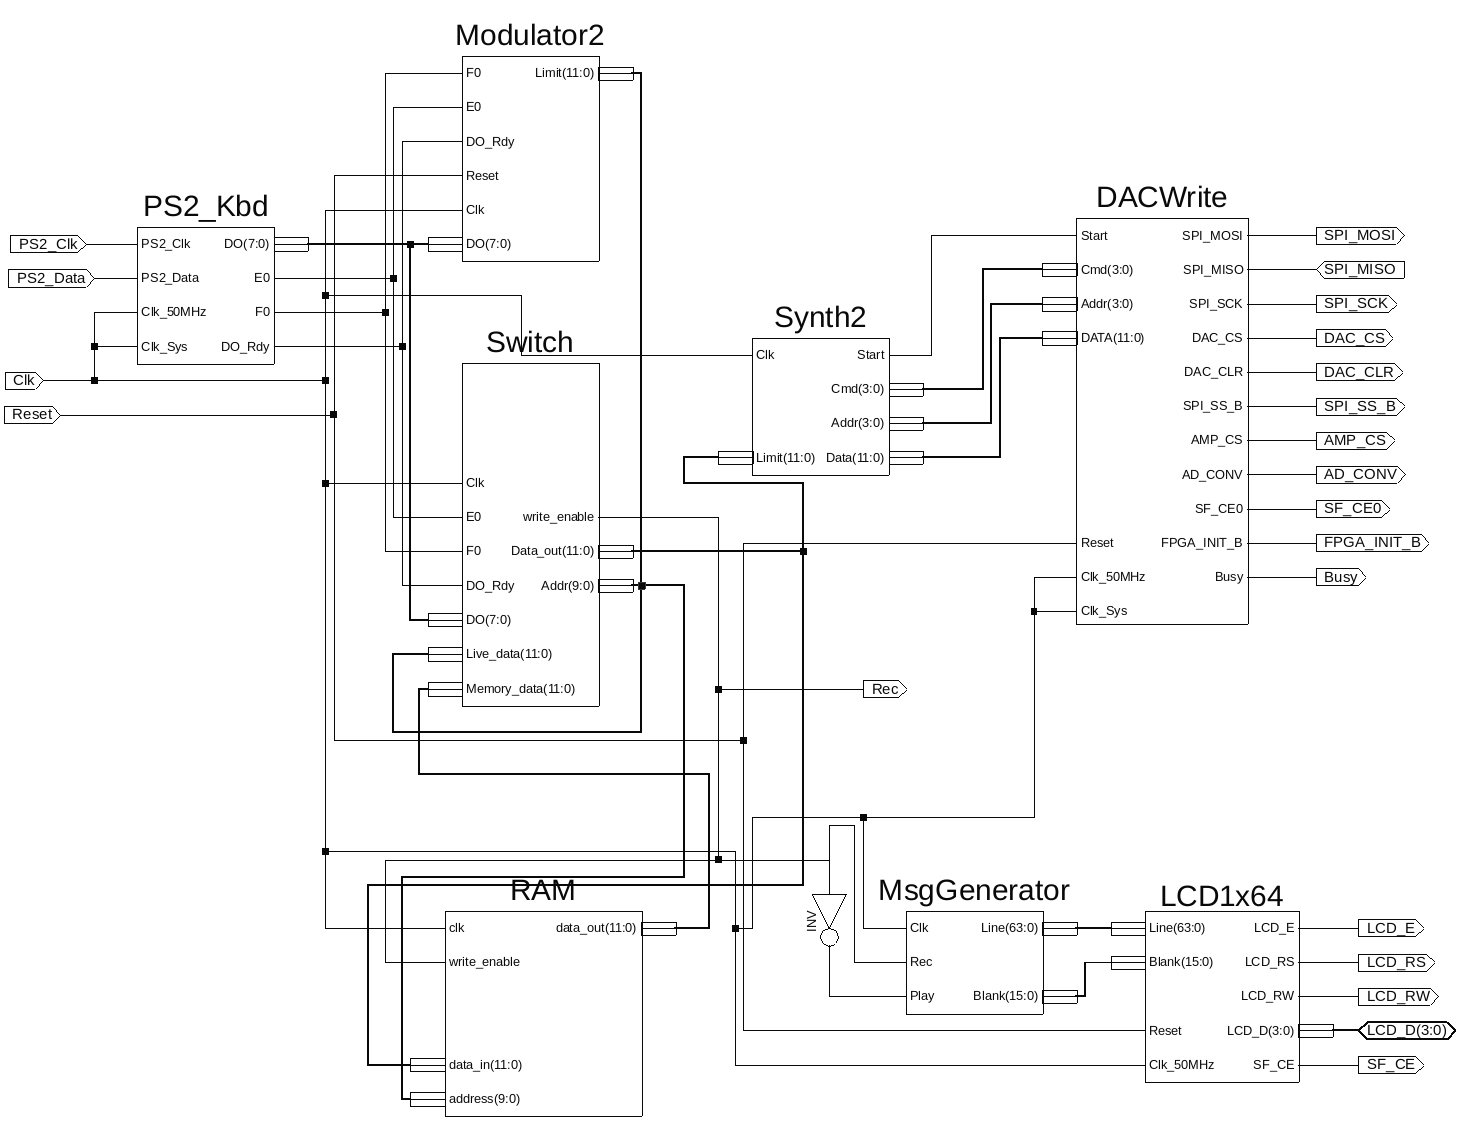
\includegraphics[scale=0.35]{schemat.png}
\caption{Schemat całego projektu.}
\end{figure}
\textbf{Hierarchia modułów:}
\begin{itemize}
\item schemat
\begin{itemize}
\item DACWrite
\item Modulator2
\item PS2_Kdb
\item Synth2
\item Switch
\item RAM
\item LCD1x64
\item MsgGenerator
\item ADC_DAC.ucf
\item GenIO.ucf
\item LCD.ucf
\end{itemize}
\end{itemize}

\subsection{Moduły}
W tym podrozdziale znajdują się opisy i symulacje modułów stworzonych na zajęciach w ramach projektu.

\subsubsection{Modulator2}
Ten moduł odpowiedzialny jest za wysyłanie wartości ograniczającej licznik w module Synth2 na podstawie sygnału pochodzącego z klawiatury. Jest oparty na maszynie stanów, która składa się 14 stanów odpowiadających różnym dźwiękom w oktawie lub ciszy.

\begin{figure}[H]
\center
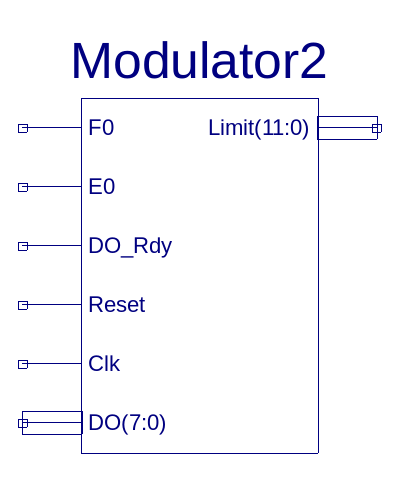
\includegraphics[scale=0.5]{modulatorSymb.png}
\caption{Symbol modułu Modulator2.}
\end{figure}

\subsubsection*{Wejścia modułu:}
\begin{itemize}
\item F0 - symbolizuje zwolnienie klawisza klawiatury
\item E0 - symbolizuje czy dane to tzw. kod rozszerzony
\item DO_Rdy - symbolizuje zakończenie odbierania kodu
\item Clk - symbolizuje zegar
\item DO[7:0] - symbolizuje otrzymane dane z klawiatury
\end{itemize}

\subsubsection*{Wyjścia modułu:}
\begin{itemize}
\item limit - symbolizuje wartość graniczną dla licznika
\end{itemize}

\subsubsection*{Fragmenty kodu VHDL}
\begin{lstlisting}[caption=Procesy modułu Modulator2.]
architecture Behavioral of Modulator2 is
   type state_type is (Silence, C, Cis, D, Dis, E, F, Fis, G, Gis, A, Ais, H, C2);
   signal state, next_state: state_type;
begin

   process1 : process( Clk )
   begin
         if rising_edge( Clk ) then
            if Reset = '1' then
               state <= Silence;
            else
               state <= next_state;
            end if;
         end if;
   end process process1;
   
   process2: process (state, DO, F0, DO_Rdy)
   begin
      next_state <= state;
      
      if DO_Rdy = '1' and F0 = '0' then
      
         case state is
            when Silence =>
               if DO = X"1C" then
                  next_state <= C;
               elsif DO = X"1D" then
                  next_state <= Cis;
               elsif DO = X"1B" then
                  next_state <= D;
               elsif DO = X"24" then
                  next_state <= Dis;
               elsif DO = X"23" then
                  next_state <= E;
               elsif DO = X"2B" then
                  next_state <= F;
               elsif DO = X"2C" then
                  next_state <= Fis;
               elsif DO = X"34" then
                  next_state <= G;
               elsif DO = X"35" then
                  next_state <= Gis;
               elsif DO = X"33" then
                  next_state <= A;
               elsif DO = X"3C" then
                  next_state <= Ais;
              elsif DO = X"3B" then
                  next_state <= H;
              elsif DO = X"42" then
                  next_state <= C2;
              end if;
              
            when C =>
               next_state <= state;
               
            when Cis =>
               next_state <= state;
               
            when D =>
               next_state <= state;
               
            when Dis =>
               next_state <= state;
            
            when E =>
               next_state <= state;
               
            when F =>
               next_state <= state;
               
           when Fis =>
               next_state <= state;
               
           when G =>
               next_state <= state;
           
           when Gis =>
               next_state <= state;
               
            when A =>
               next_state <= state;
               
            when Ais =>
               next_state <= state;
               
            when H =>
               next_state <= state;
               
            when C2 =>
               next_state <= state;
         end case;
      elsif F0 = '1' then
         next_state <= Silence;
      end if;
   end process process2;
   
   with state select
      Limit <= X"5D4" when C,
               X"581" when Cis,
               X"532" when D,
               X"4E7" when Dis,
               X"4A1" when E,
               X"45E" when F,
               X"41F" when Fis,
               X"3E4" when G,
               X"3AC" when Gis,
               X"377" when A,
               X"345" when Ais,
               X"316" when H,
               X"2EA" when C2,
               X"000" when others;

end Behavioral;
\end{lstlisting}
Architektura jednostki na samym początku posiada deklarację wszystkich stanów, które odpowiadają dźwiękom w oktawie lub ciszy.
Pierwszy proces jest typowym przykładem procesu odpowiedzialnego za przełączanie stanu w maszynie stanów. Kolejny proces odpowiada za wybranie odpowiedniego stanu w zależności od wciśniętego klawisza. Ostatni element modułu to ustawianie odpowiedniego limitu w zależności od aktualnego stanu.

\subsubsection*{Graf maszyny stanu}
\begin{figure}[H]
\center
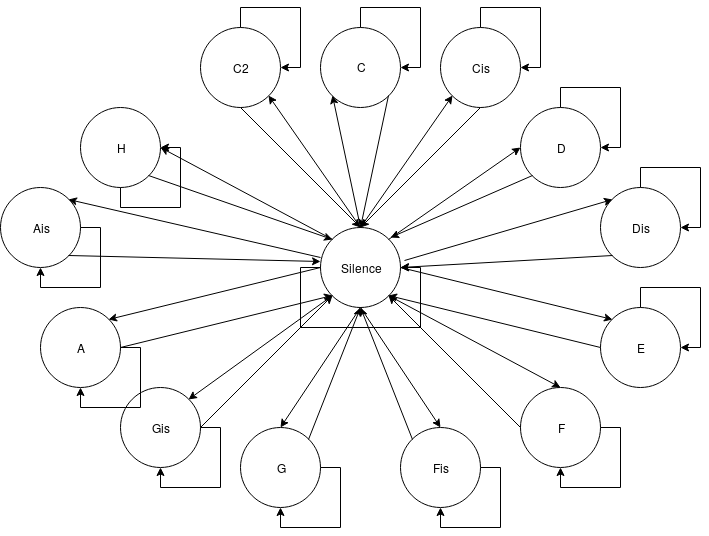
\includegraphics[scale=0.6]{modulatorMaszyna.png}
\caption{Graf maszyny stanów modułu Modulator2.}
\end{figure}

\subsubsection*{Symulacja}
\begin{figure}[H]
\center
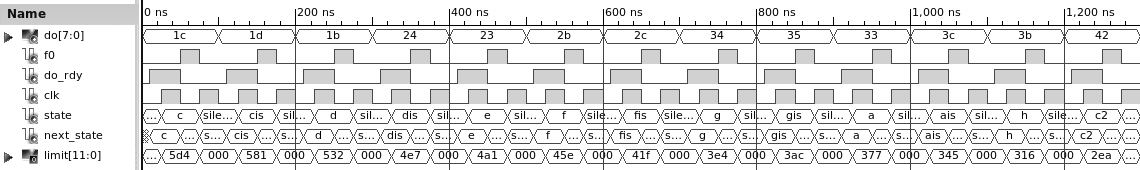
\includegraphics[scale=0.6]{modulatorsymbw.png}
\caption{Wyniki symulacji modułu Modulator2.}
\end{figure}
Na powyższej symulacji widać jak w momencie impulsu sygnału do_rdy z najbliższym taktem zegara zmieniany jest stan maszyny zgodnie z wciśniętym klawiszem oraz ustawiany jest odpowieni limit. W momencie impulsu f0 (puszczenie klawisza) stan przełączany jest na silence, a limit na wartość zerową.

\subsubsection{Synth2}

\subsubsection{Switch}

\subsubsection{RAM}

\subsubsection{MsgGenerator}

\section{Implementacja}
\subsection{Zasoby}
\subsection{"User manual" urządzenia}

\section{Podsumowanie}
Zadanie udało się zrealizować w całości. Instrument jest w pełni działający, a ze względu na jasny podział na moduły można bez trudu dopisywać do niego kolejne funkcjonalności. Także sama wartość "merytoryczna" keyboarda nie pozostawia wiele do życzenia, ponieważ faktycznie pokrywa on całą oktawę, a wysokości dźwięków różnią się od siebie dokładnie tak jak w prawdziwym instrumencie, dzięki czemu mając nuty do utworu muzycznego możemy go zagrać.

\section{Literatura}

\end{document}

